\begin{answer}

    \begin{figure}[h]
        \centering
        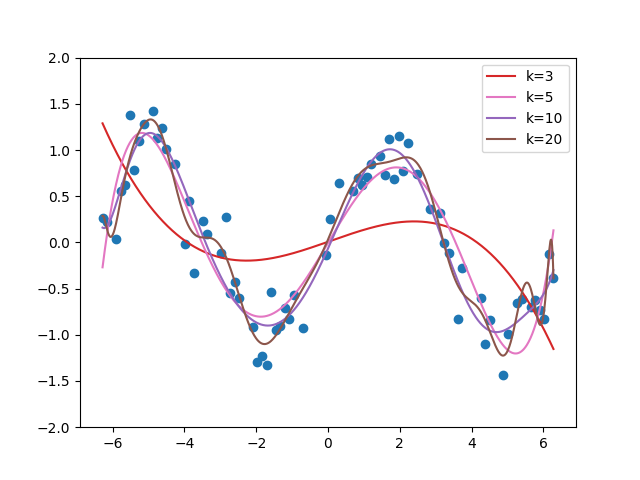
\includegraphics[width=0.8\textwidth]{src/featuremaps/plot-degrees[3, 5, 10, 20].png}
        \caption{Polynomial regression with multiple degrees}
        \label{fig:degree3}
    \end{figure}

    The higher the polynomial degree gets, and the more features we get, the higher the variance gets and the more the curve overfits. It can model now more information, but with that also starts to learn the noise that comes with each sample and doesn't generalize as well anymore (high variance, low bias)
\end{answer}
